% ---------
%  Compile with "pdflatex hw1".
% --------
%!TEX TS-program = pdflatex
%!TEX encoding = UTF-8 Unicode

% Template borrowed from Jeff Erickson.

\documentclass[11pt]{article}
\usepackage[utf8]{inputenc}		% Allow some non-ASCII Unicode in source
\usepackage{jeffe, handout,graphicx}
\usepackage{forest}
\usepackage{mathtools}
\usepackage{tikz, ifthen, etoolbox}
\usepackage{float}
\usetikzlibrary{positioning}
\newcommand{\pd}{\partial}
\newcommand{\bs}{\boldsymbol}
\newcommand{\ifstringequal}[4]{%
  \ifnum\pdfstrcmp{#1}{#2}=0
  #3%
  \else
  #4%
  \fi
}


% =========================================================
%   Define common stuff for solution headers
% =========================================================
\Class{CS 6301.503}
\Semester{Spring 2019}
\Authors{1}
\AuthorOne{Scott C. Waggener}{scw180000}
%\Section{}
% =========================================================
\begin{document}
\HomeworkHeader{4 (Probability)}{1}% homework number, problem number
% ---------------------------------------------------------
Complete

% =========================================================
\HomeworkHeader{4 (Probability)}{2}% homework number, problem number
% ---------------------------------------------------------
Complete

% =========================================================
\HomeworkHeader{4 (Probability)}{3}% homework number, problem number
% ---------------------------------------------------------
\noindent
\begin{enumerate}[(a)]\itemsep0pt
\item You're person B and want to win, which version of the game do you play?
	\begin{solution}
		The standard version
	\end{solution}

	\begin{proof}
		Think of this in terms of maximizing information gain with each
		question. If we do not receive an answer immediately after each
		question our best strategy would be to choose the top $20$ questions
		that provide the most mutual information about the object without
		considering how information gain at a given question is conditioned on
		the answer of previous questions.
		\newline

		If we do receive an answer after each question, we can choose
		information maximizing questions conditioned on known realizations of the
		random variables given as answers.
	\end{proof}

\item
	\begin{solution}
		The modified game
	\end{solution}
	\begin{proof}
		The input tensor passes through multiple layers before being converted
		to a feature vector. The dense layer then uses this feature vector to
		eventually provide a class pmf vector. In this construction the feature
		vector can be thought of as answers to the $20$ questions which are
		used to compute each class probability. There is no dependency on which
		features a network extracts at a given layer conditioned on the
		features extracted from a previous layer.
	\end{proof}

\item
	\begin{solution}
		Essentially, provide redundancy assuming the probability of an
		incorrect answer is not $0.5$.
	\end{solution}
	\begin{proof}
		Of course, if we are given an incorrect answer with probability $0.5$
		we have an entropy maximizing uniform distribution across both possible
		answers. We will receive no information from each answer and will be
		unable to play the game.
		\newline

		Otherwise, we can attempt to provide some redundancy in our questions
		to help minimize the uncertainty about answers. We can tailor the
		amount of overlap based on the probability of receiving a correct or
		incorrect answer, with greater overlap required as the probabilities
		approach $0.5 / 0.5$. Furthermore, we can trivially handle the case
		where we are more likely to receive an incorrect answer by negating the
		given answer.
		\newline

		The chain rule can be written as

		\begin{align}
			p\Big( x_{n-1} \vert \hat x_{n-2}, \hat x_{n-3}, \dots,
				\hat x_{0}\Big)
			&= \frac{
			p\Big( x_{n-1}, \hat x_{n-2}, \hat x_{n-3}, \dots,
				\hat x_{0}\Big)
			}{
			p\Big(\hat x_{n-2}, \hat x_{n-3}, \dots,
				\hat x_{0}\Big)
			}
		\end{align}

		Tweaking the overlap of questions would exert control over the joint
		probability seen in the denominator (and partially in numerator).

	\end{proof}

\item
	\begin{solution}
		Strategy change is similar to the one used for the original game, but
		providing redundancy blindly during the questioning process.
	\end{solution}
	\begin{proof}
		Now we are playing the modified game, but with some probability the
		given answer will be wrong. At the end of the round we will have a
		probability for each class conditioned on $20$ answers which are only
		correct with some probability. Again, we wouldn't play with a $0.5 /
		0.5$ probability split since each answer provides no information.
		Otherwise we need to provide some redundancy in our questions, but we
		cannot determine the best redundancy providing questions conditioned on
		answers to other questions.
		\newline

		Since our answers are only correct with some probability we cannot
		exclude any classes from our output pmf. Additionally, a network would
		provide this redundancy by extracting multiple features that may point
		to a given class. Since each extracted feature may be incorrect, having
		multiple features that indicate membership to a given class provides
		redundancy.

	\end{proof}

\end{enumerate}
% =========================================================
\HomeworkHeader{4 (Probability)}{4}
% ---------------------------------------------------------
\begin{solution}
	The plot was generated using $100$ trials for each of the possible number
	of known questions. Sampling was done using $\texttt{np.random.binomial}$
	with $n=1,\ p=0.25,\ \text{size}=(100 - \text{known})$
	\begin{figure}[H]
		\centering
		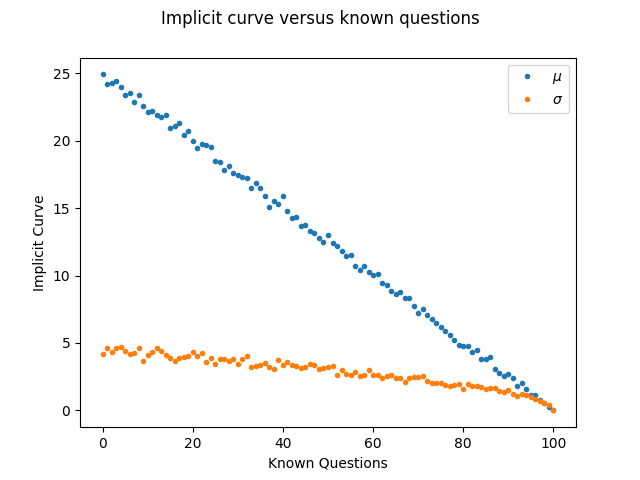
\includegraphics[width=0.8\linewidth]{figures/q4.png}
		\caption{Implicit curve $\mu, \sigma$ versus number of known questions.}
	\end{figure}

\end{solution}


% =========================================================
\HomeworkHeader{4 (Probability)}{5}
% ---------------------------------------------------------
Assume ImageNet has 1.28 million images of size 3 x 256 x 256 with 1280 images
each in 1000 different classes. How many bits of information are in the ImageNet
labels?

\begin{solution}
	$10$ bits
\end{solution}

\begin{proof}
	Since entropy can informally be defined as the information in the
	realization of a random variable, we can compute the entropy for the given
	problem. We have $1280$ images in each of the $1000$ classes, meaning
	\begin{align}
		H(x(s)) &= -\Sum_{i=1}^{1000} \frac{1}{1000}\log_2\left(
			\frac{1}{1000}\right)
		\\
		&= -\frac{1000}{1000} \log_2\left(\frac{1}{1000}\right)
		\\
		&= \log_2 1000
		\\
		&\approx 9.97
	\end{align}
\end{proof}


\end{document}
